%%%%%%%%%%%%%%%%%%%%%%%%%%%%%%%%%%%%%%%%%%%%%%%%%%%%%%%%%%%%%%%%%%%%%%%%%%%%%%%%
\section{Wymagania funkcjonalne}
%%%%%%%%%%%%%%%%%%%%%%%%%%%%%%%%%%%%%%%%%%%%%%%%%%%%%%%%%%%%%%%%%%%%%%%%%%%%%%%%

Projektowanie systemu informatycznego, zgodnie z założeniami inżynierii oprogramowania, rozpoczyna się od ustalenia wymagań funkcjonalnych, które powinno spełniać tworzone oprogramowanie. Wymagania te formułują zakres czynności, do których, zdolni są użytkownicy, podczas eksploatacji systemu:

\begin{itemize}
    \item Użytkownik nieuwierzytelniony posiada możliwość utworzenia konta w systemie.
    \item Użytkownik nieuwierzytelniony posiada możliwość uwierzytelnienia się, za pomocą wcześniej utworzonego konta. Jest to czynność mająca na celu, uzyskanie autoryzacji do skorzystania z reszty funkcjonalności systemu.
    \item Użytkownik uwierzytelniony może w prosty sposób, przeglądać jedną z tabel przypisanych do niego zasobów. Wyróżniamy tabele członków drużyny, sprzętu spalinowego oraz odbytych akcji.
    \item Użytkownik uwierzytelniony jest w stanie utworzyć jedną encję zasobu w przeglądanej tabeli przy pomocy formularza edycji.
    \item Użytkownik uwierzytelniony jest w stanie edytować jedną encję zasobu w przeglądanej tabeli przy pomocy formularza edycji.
    \item Użytkownik uwierzytelniony jest w stanie zaznaczyć jedną lub wiele encji zasobów w przeglądanej tabeli.
    \item Użytkownik uwierzytelniony jest w stanie permanentnie usunąć jedną lub wiele zaznaczonych encji zasobów w przeglądanej tabeli.
    \item Użytkownik uwierzytelniony ma możliwość stworzenia encji zasobu odbytej akcji, bazując na zaznaczonych członkach zespołu i sprzętu pożarowego. Formularz tworzonej akcji zawiera wtedy dodatkowe pola, pozwalające na uzupełnienie roli poszczególnych członków brygady oraz poziomu zużytego paliwa dla wybranego sprzętu.
    \item Użytkownik uwierzytelniony ma możliwość natychmiastowego usunięcia danych uwierzytelniających, z pamięci przeglądarki internetowej.
\end{itemize}

%%%%%%%%%%%%%%%%%%%%%%%%%%%%%%%%%%%%%%%%%%%%%%%%%%%%%%%%%%%%%%%%%%%%%%%%%%%%%%%%
\section{Wymagania jakościowe}
%%%%%%%%%%%%%%%%%%%%%%%%%%%%%%%%%%%%%%%%%%%%%%%%%%%%%%%%%%%%%%%%%%%%%%%%%%%%%%%%

Celem, postawionych systemowi wymagań jakościowych, jest uczynienie go łatwiejszym w obsłudze dla jego użytkowników. Spełnienie tych wymagań, ma na celu zwiększenie zadowolenia użytkownika z funkcjonalności, jakie oferuje system. Jako dodatkowy efekt, można uznać łatwiejszy rozwój systemu w procesie produkcyjnym: 

\begin{itemize}
    \item Aplikacja kliencka systemu powinna funkcjonować poprawnie z wykorzystaniem nowoczesnych przeglądarek internetowych takich jak Microsoft Edge, Google Chrome, Mozilla Firefox i Safari.
    \item Aplikacja kliencka powinna reagować na zmianę rozdzielczości ekranu urządzenia i wyświetlać się poprawnie, niezależnie od jego proporcji.
    \item Aplikacja kliencka będzie informowała o awariach i błędach w systemie w sposób jasny i zrozumiały dla użytkownika.
    \item Aplikacja kliencka ma wymagać potwierdzenia krytycznych i nieodwracalnych akcji.
    \item Wymagana jest walidacja danych w formularzach, zarówno po stronie aplikacji klienckiej jak i serwerowej.
    \item System będzie rozwijany w języku angielskim, zgodnie ze standardem rynku oprogramowania.
\end{itemize}

%%%%%%%%%%%%%%%%%%%%%%%%%%%%%%%%%%%%%%%%%%%%%%%%%%%%%%%%%%%%%%%%%%%%%%%%%%%%%%%%
\section{Diagram przypadków użycia}
%%%%%%%%%%%%%%%%%%%%%%%%%%%%%%%%%%%%%%%%%%%%%%%%%%%%%%%%%%%%%%%%%%%%%%%%%%%%%%%%

Kolejnym etapem po ustaleniu wymagań, które powinien spełnić system, powinno być sporządzenie diagramu UML przypadków użycia. Diagram ten ma na celu, przedstawienie rodzajów użytkowników oraz ich możliwości nawiązania interakcji z systemem.

Najważniejszymi elementami diagramu są jego aktorzy. Aktor najczęściej jest reprezentacją typu użytkownika systemu, jednakże w nowszych specyfikacjach UML 2.0 wyodrębnione zostały również oznaczenia przeznaczone dla aktorów, będących podsystemami lub zewnętrznymi modułami, współpracującymi z projektowanym systemem. Ze względu na nieduży zakres obowiązków tworzonego prototypu, wyróżnione zostały dwa typy aktorów, wchodzących w interakcje z aplikacją.

\begin{itemize}
    \item Użytkownik nieuwierzytelniony - nie posiada konta lub nie uwierzytelnił się w systemie. Dla aktora tego typu, nie są dostępne żadne funkcjonalności oprócz akcji uwierzytelnienia się lub założenia nowego konta. Przed manipulacją zasobami powstrzymują go mechanizmy autoryzacji.
    \item Użytkownik uwierzytelniony - ma możliwość skorzystania ze wszystkich funkcji systemu związanych z zasobami i akcjami OSP.
\end{itemize}

W przypadku dalszego rozwoju aplikacji, naturalnym krokiem byłoby stworzenie hierarchii użytkowników uwierzytelnionych. W zależności od roli danego aktora, posiadałby on unikalne dla swojej podgrupy przywileje i uprawnienia do skorzystania z akcji, dostępnych w ramach aplikacji.

Aby zapewnić większą czytelność tworzonego diagramu, inżynierowie oprogramowania decydują się na podział, przedstawianych przypadków użycia na moduły funkcjonalne. Moduły te, oddzielają od siebie niepowiązane ze sobą funkcjonalności, pozwalając na wstępny podział systemu na mniejsze części składowe. W tworzonej aplikacji, wyodrębnione zostały dwa moduły, najważniejsze dla potencjalnych użytkowników:

\begin{itemize}
    \item Users - moduł poświęcony funkcjonalnościom tworzenia kont użytkowników oraz ich uwierzytelnianiu.
    \item Resources - obejmujący funkcje związane z manipulacją zasobami uwierzytelnionego użytkownika. Przykładowymi akcjami, możliwymi do wykonania w ramach modułu są: dodanie, usunięcie i modyfikacja danego zasobu.
\end{itemize}

Uwzględniając przeprowadzoną analizę aktorów oraz wymagań funkcjonalnych systemu, sporządzony został diagram przypadków użycia przedstawiony na rys. \ref{fig:uml.use-case}. Jest to klarowna i zrozumiała dla każdego inżyniera oprogramowania, podstawa dalszego projektowania bardziej szczegółowych elementów składowych systemu.

\begin{figure}[!htbp] 
    \centering
    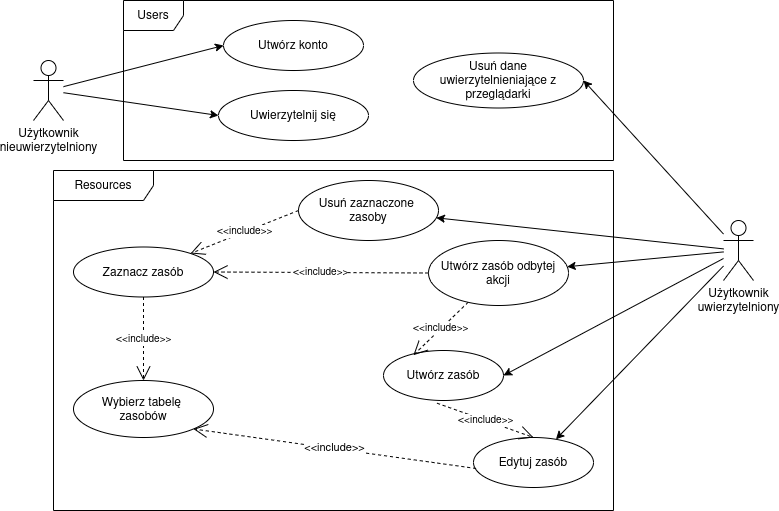
\includegraphics[width=\textwidth]{img/chapter4/open-osp.uml-diagrams-use-case.png}
    \caption{Diagram przypadków użycia}
    \label{fig:uml.use-case}
\end{figure}

%%%%%%%%%%%%%%%%%%%%%%%%%%%%%%%%%%%%%%%%%%%%%%%%%%%%%%%%%%%%%%%%%%%%%%%%%%%%%%%%
\section{Diagram klas encji}
%%%%%%%%%%%%%%%%%%%%%%%%%%%%%%%%%%%%%%%%%%%%%%%%%%%%%%%%%%%%%%%%%%%%%%%%%%%%%%%%

W celu zaprojektowania podstawowych struktur danych, biorących udział w procesach logicznych systemu, sklasyfikowano przechowywane w bazie danych encje:

\begin{itemize}
    \item User - obiekt opisujący konto założone przez użytkownika aplikacji. Zawiera atrybuty adresu e-mail, będącego identyfikatorem użytkownika w procesie uwierzytelniającym oraz zaszyfrowaną wersję hasła.
    \item Member - obiekt członka jednostki strażackiej mogącego brać udział w akcjach. W podstawowej wersji systemu, członek drużyny jest opisany przez atrybuty swojego imienia, nazwiska i numeru PESEL. W dalszym procesie rozwoju aplikacji, należałoby rozważyć dodanie atrybutów takich jak ranga, zdobyte odznaczenia czy termin następnych badań okresowych.
    \item Equipment - obiekt reprezentujący sprzęt, wchodzący w inwentarz jednostki, taki jak samochody, piły spalinowe lub węże strażackie. Dla uproszczenia tworzonego prototypu, zdecydowano się na jedną klasę opisującą użyteczne przedmioty, przy pomocy atrybutów nazwy własnej, marki, modelu i numeru seryjnego (pełniącego również rolę numerów rejestracyjnych dla pojazdów spalinowych). 
    \item Action - obiekt akcji strażackiej opisujący ją przy pomocy atrybutów jej typu i lokacji podanej przy pomocy szerokości oraz długości geograficznej. Każda z akcji będzie miała również swój czas rozpoczęcia i zakończenia.
    \item ActionMember - obiekt opisujący rolę danego członka zespołu w odbytej akcji. Jego atrybutami są unikalne numery identyfikujące członka jednostki oraz akcji, w której bierze on udział. Rola członka zespołu jest określana przy pomocy, przeznaczonego w tym celu typu wyliczeniowego.
    \item ActionEquipment - obiekt opisujący eksploatacje sprzętu  w odbytej akcji. Pierwszorzędnymi atrybutami encji są unikalne identyfikatory odbytej akcji oraz sprzętu strażackiego. Jego zużycie można opisać dodatkowo atrybutami ilości zużytych litrów paliwa oraz stanu licznika po akcji.
\end{itemize}

W procesie opisywania klas, wyodrębniono dodatkowe dwa typy numeryczne. Typy te pozwalają na bardziej klarowny sposób zarządzania informacjami zapisanymi przy pomocy pojedynczej liczby całkowitej:

\begin{itemize}
    \item ActionType - typ wyliczeniowy określający rodzaj odbytej akcji. Wśród możliwych wartości wyróżniono: wyjazd zaopatrzeniowy, akcję treningową, akcję pożarniczą i zwalczanie innych zagrożeń/klęsk żywiołowych.
    \item ActionMemberRole - określa rolę członka drużyny uczestniczącego w akcji. Członek drużyny może zostać rozróżniony jako: zwykły członek zespołu, kierowca lub dowódca.
\end{itemize}

Typy wyliczeniowe, stanowią bardzo pożyteczne narzędzie w programowaniu wysokopoziomowym, pozwalając na  oszczędność pamięci i ograniczenie złożoności obliczeniowej, względem typów takich jak łańcuch znaków. Zapewniają również, bardzo korzystną dla inżynierów oprogramowania, skalowalność tworzonego rozwiązania.

Stworzony na podstawie przeprowadzonej analizy, diagram klas UML został przedstawiony na rys. \ref{fig:uml.classes}. Stanowi on przejrzysty projekt warstwy modelu danych systemu, umożliwiając rozpoczęcie prac nad logiką biznesową. Diagramy klas stanowią najpopularniejsze diagramy UML, stosowane w inżynierii oprogramowania, należące do podzbioru diagramów strukturalnych.

\begin{figure}[!htbp]
    \centering
    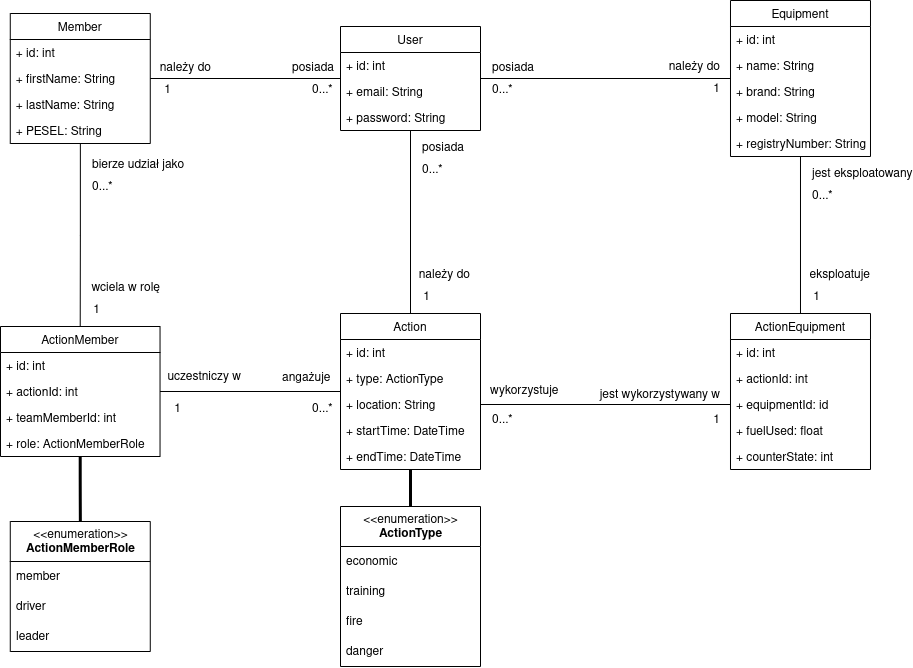
\includegraphics[width=\textwidth]{img/chapter4/open-osp.uml-diagrams-classes.png}
    \caption{Diagram klas encji}
    \label{fig:uml.classes}
\end{figure}

%%%%%%%%%%%%%%%%%%%%%%%%%%%%%%%%%%%%%%%%%%%%%%%%%%%%%%%%%%%%%%%%%%%%%%%%%%%%%%%%
\section{Diagram aktywności}
%%%%%%%%%%%%%%%%%%%%%%%%%%%%%%%%%%%%%%%%%%%%%%%%%%%%%%%%%%%%%%%%%%%%%%%%%%%%%%%%

Projektowanie warstwy logiki systemu, rozpoczęto od stworzenia diagramu aktywności. Diagram ten, stanowi jeden z najpopularniejszych sposobów, przedstawienia przebiegu interakcji między użytkownikiem, a oprogramowaniem. Jako przedstawiciel zbioru diagramów zachowań, jest powiązany z przedstawionym na rys. \ref{fig:uml.use-case} diagramem przypadków użycia, wyróżniając się dodatkowymi oznaczeniami dla podejmowanych decyzji i ciągłością przebiegu.

\begin{figure}[!htbp]
    \centering
    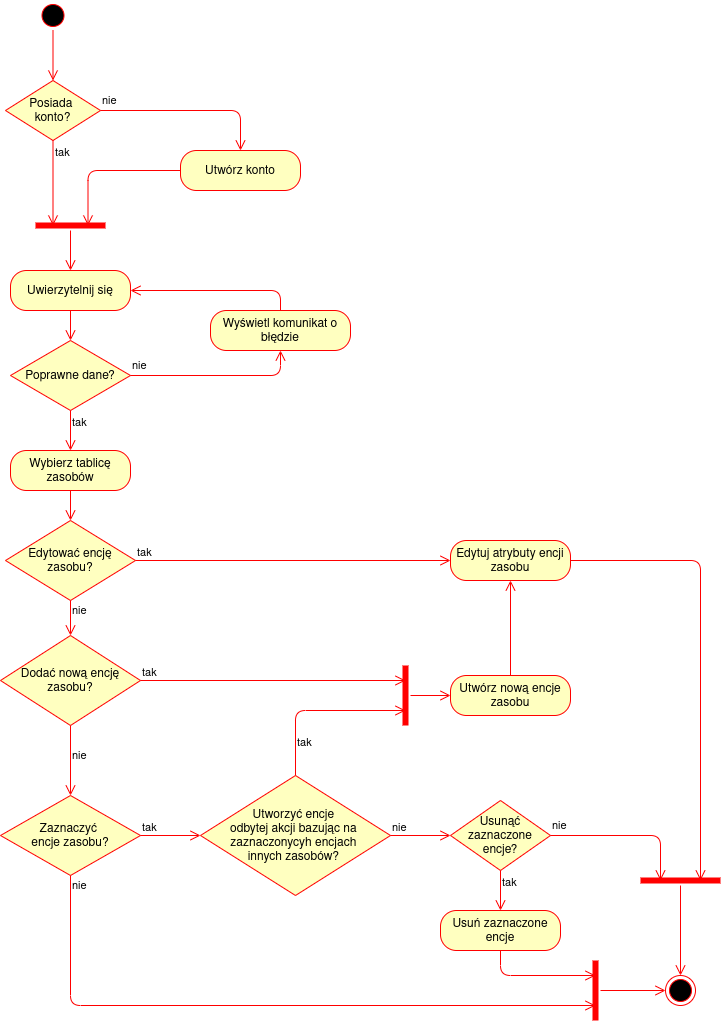
\includegraphics[width=\textwidth]{img/chapter4/open-osp.uml-diagrams-activity.png}
    \caption{Diagram aktywności}
    \label{fig:uml.activity}
\end{figure}

Diagram aktywności przedstawiony na rys. \ref{fig:uml.activity} jest szczególnie przydatny przy planowaniu ilości i przeznaczenia widoków w aplikacji klienckiej. W celu przedstawienia szczegółowego cyklu życia zasobów, przypisanych do użytkownika systemu, zastosowano diagramy sekwencji opisane w dalszej sekcji.

%%%%%%%%%%%%%%%%%%%%%%%%%%%%%%%%%%%%%%%%%%%%%%%%%%%%%%%%%%%%%%%%%%%%%%%%%%%%%%%%
\section{Widoki aplikacji klienckiej}
%%%%%%%%%%%%%%%%%%%%%%%%%%%%%%%%%%%%%%%%%%%%%%%%%%%%%%%%%%%%%%%%%%%%%%%%%%%%%%%%

Bazując na diagramie aktywności, wyróżniono widoki aplikacji, stanowiące interfejs między użytkownikiem, a dostarczanymi przez system funkcjonalnościami. Warstwę widoku aplikacji tworzą niżej opisane składowe:

\begin{itemize}
    \item Strona tytułowa aplikacji, zawierająca odnośniki do widoku uwierzytelnienia i rejestracji użytkowników.
    \item Widok formularza uwierzytelnienia, składającego się z pola do wprowadzenia e-maila oraz hasła użytkownika.
    \item Widok rejestracji użytkowników, zawierający formularz do wprowadzenia danych.
    \item Widok panelu użytkownika, umożliwiającego wybór przeglądanej tabeli zasobów. W jego skład wchodzi tabela, w której każda z krotek posiada pole zaznaczenia i przycisk edycji.
    \item Widok edycji atrybutów zasobu przy pomocy pojawiającego się monitu, jednocześnie pełni funkcję widoku służącego do inicjalizacji atrybutów nowo powstałej encji.
    \item Widok edycji encji odbytej akcji. Formularz rozbudowany jest o sekcje, pozwalające uzupełnić informacje o członkach drużyny i sprzęcie, który wziął udział w akcji.
    \item Widok ostrzeżenia przed usunięciem, zaznaczonych w tabeli zasobów.
\end{itemize}

\begin{figure}[!htbp]
\centering
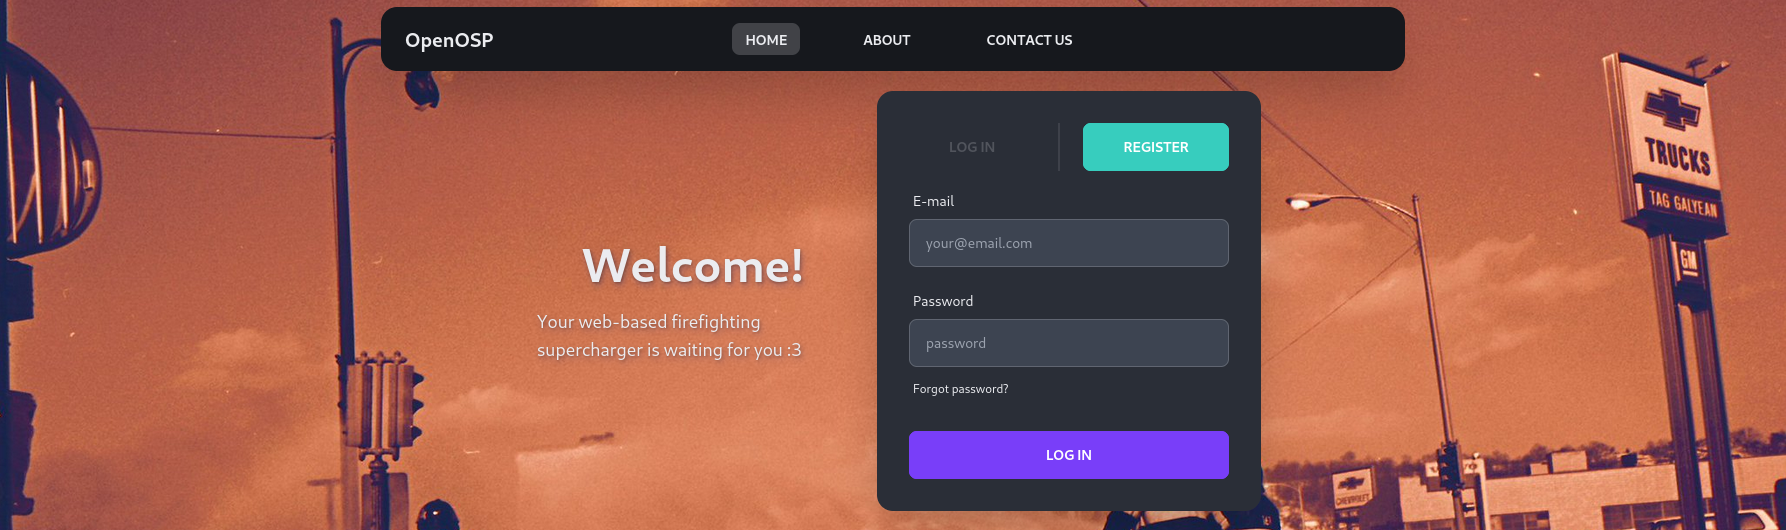
\includegraphics[width=\textwidth]{img/chapter4/views/login.png}
\caption{Widok formularza uwierzytelnienia użytkownika}
\end{figure}

\begin{figure}[!htbp]
\centering
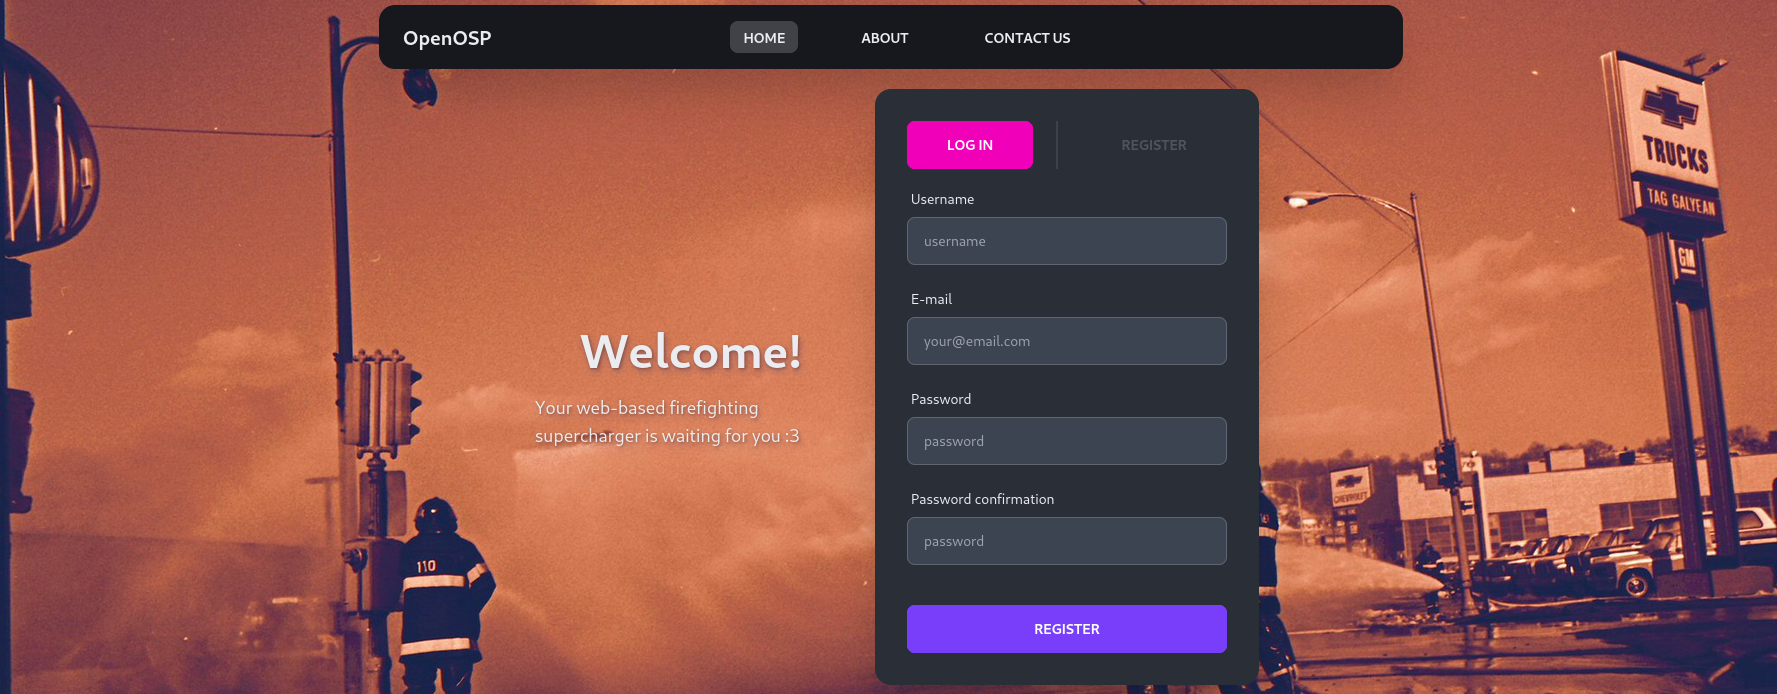
\includegraphics[width=\textwidth]{img/chapter4/views/registration.png}
\caption{Widok formularza rejestracji użytkownika}
\end{figure}

\begin{figure}[!htbp]
\centering
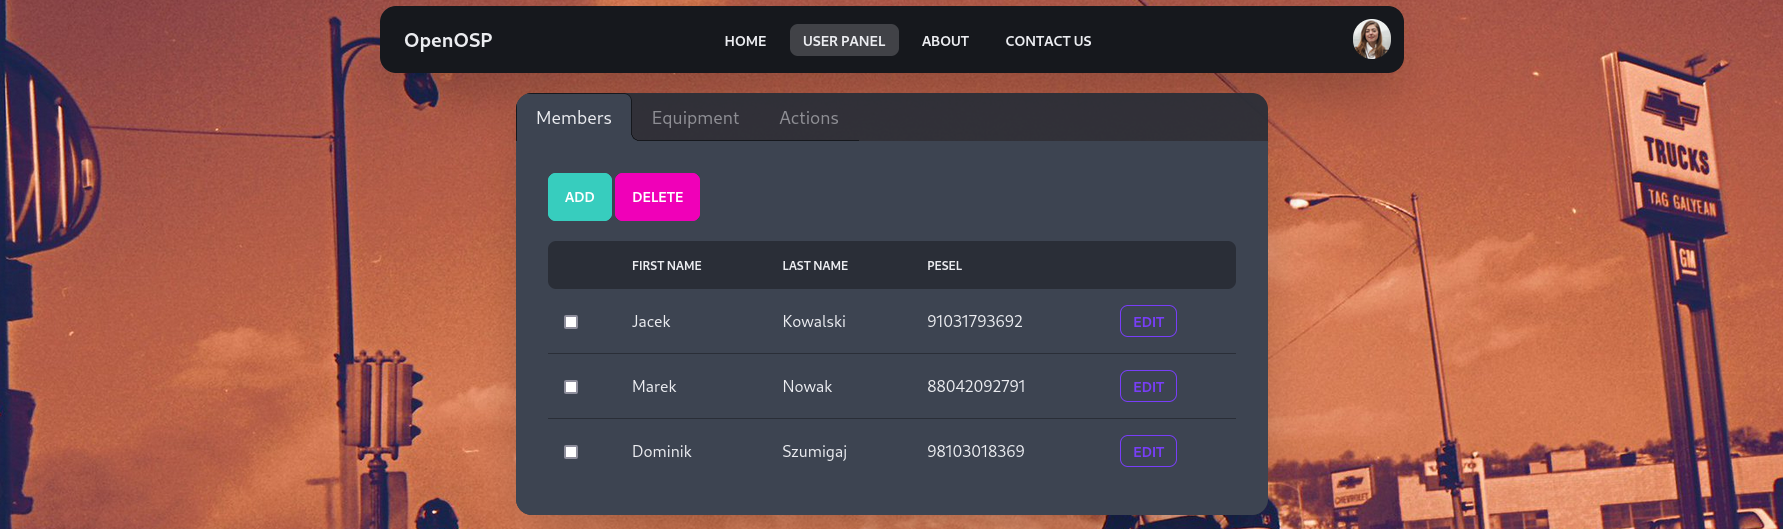
\includegraphics[width=\textwidth]{img/chapter4/views/userpanel.png}
\caption{Widok tabeli zasobów użytkownika}
\end{figure}

\begin{figure}[!htbp]
\centering
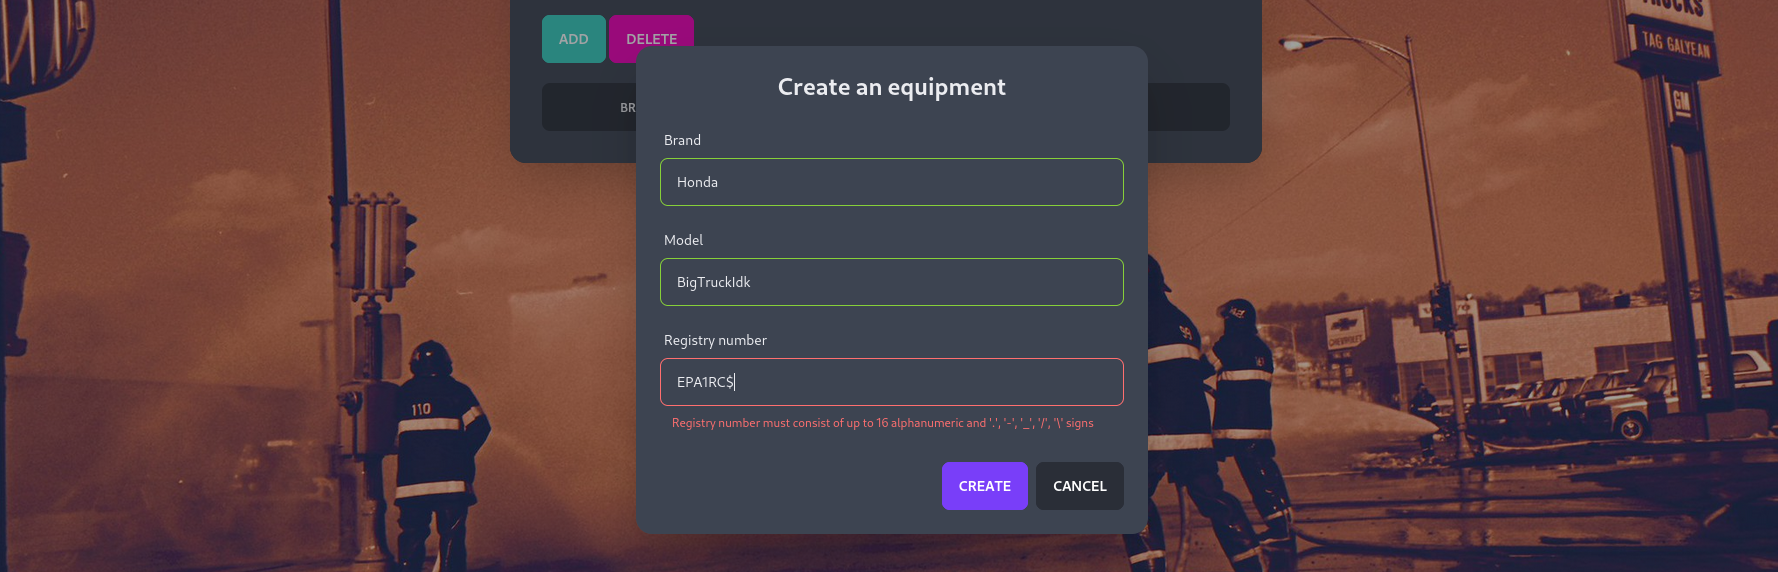
\includegraphics[width=\textwidth]{img/chapter4/views/create.png}
\caption{Widok monitu tworzenia lub modyfikacji zasobu}
\end{figure}

\begin{figure}[!htbp]
\centering
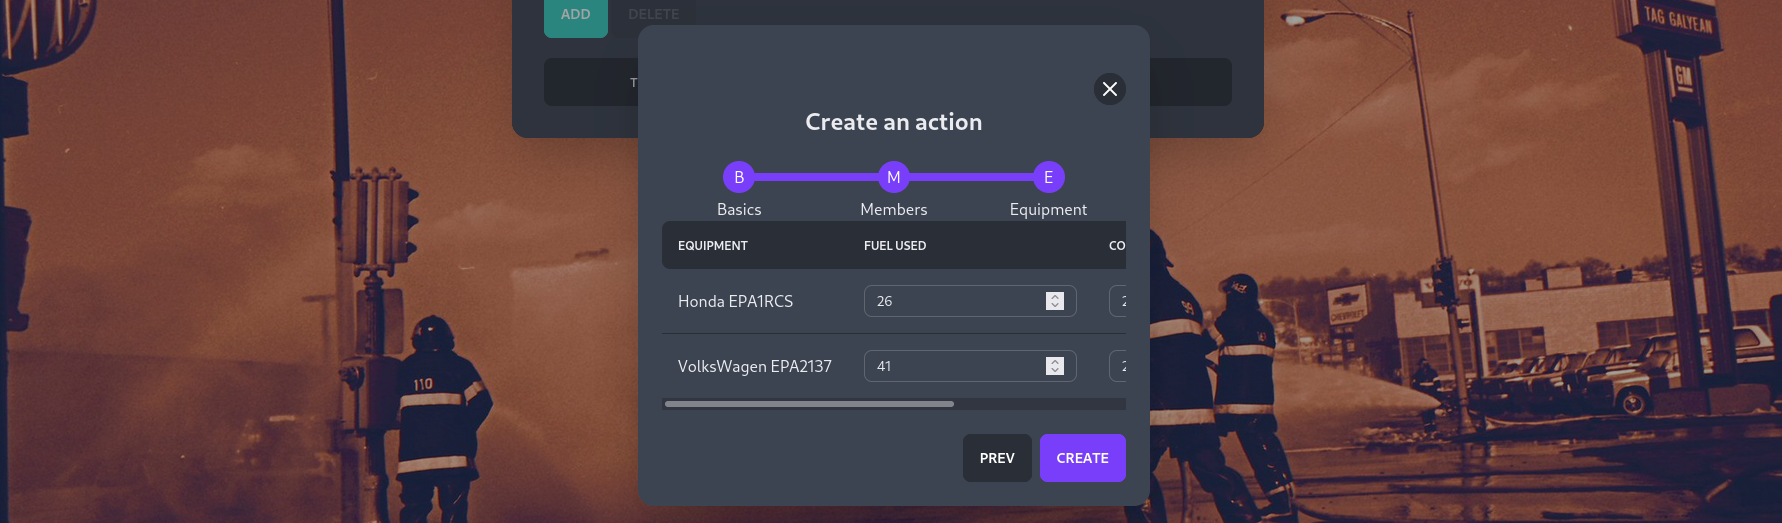
\includegraphics[width=\textwidth]{img/chapter4/views/action.png}
\caption{Widok monitu tworzenia lub modyfikacji zasobu odbytej akcji}
\end{figure}

\begin{figure}[!htbp]
\centering
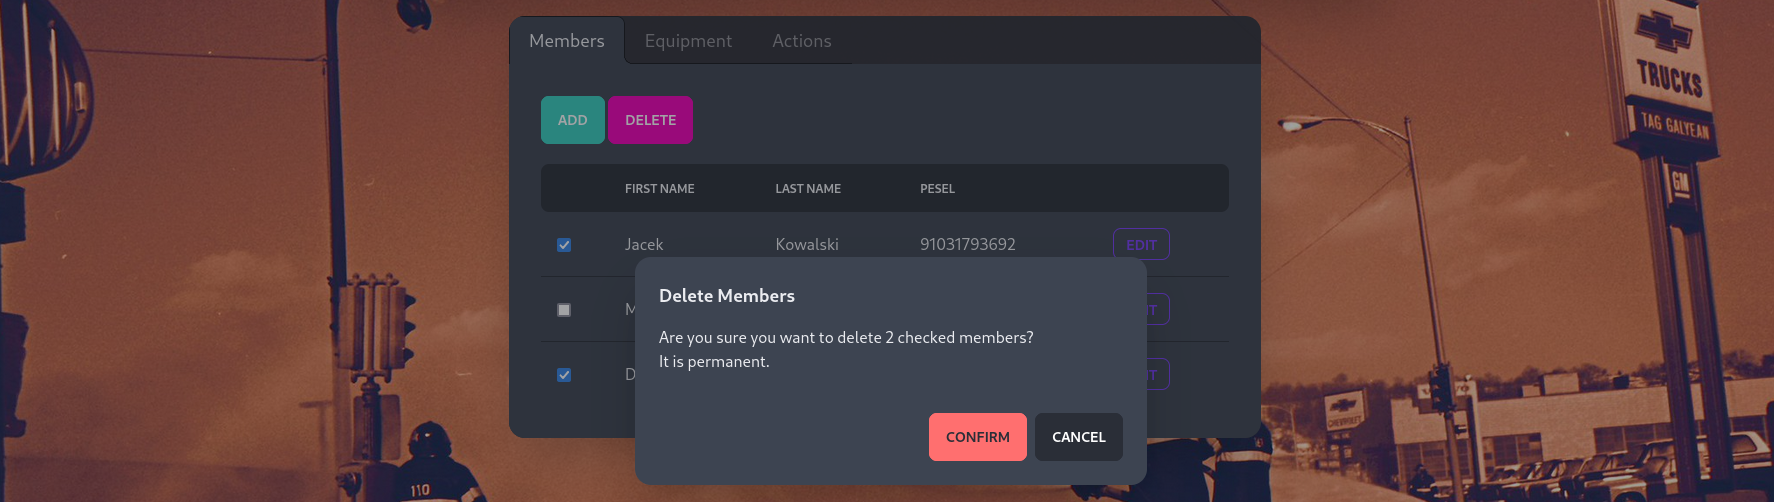
\includegraphics[width=\textwidth]{img/chapter4/views/delete.png}
\caption{Widok monitu ostrzeżenia przed usunięciem zasobów}
\end{figure}

W każdym z widoków, użytkownik ma dostęp do paska nawigacyjnego zawierającego odnośniki do panelu użytkownika oraz przycisk do wylogowania się z aplikacji. 

%%%%%%%%%%%%%%%%%%%%%%%%%%%%%%%%%%%%%%%%%%%%%%%%%%%%%%%%%%%%%%%%%%%%%%%%%%%%%%%%
\section{Cykl życia zasobu użytkownika}
%%%%%%%%%%%%%%%%%%%%%%%%%%%%%%%%%%%%%%%%%%%%%%%%%%%%%%%%%%%%%%%%%%%%%%%%%%%%%%%%

Procesy, związane z przetwarzaniem obiektów zasobów użytkownika, zostały wyodrębnione jako najważniejszy element logiczny tworzonego systemu. Z tego względu, użyto diagramów sekwencji przy projektowaniu tych funkcjonalności systemu.

Diagramy sekwencji, stanowią jedne z najbardziej szczegółowych diagramów zachowań UML, pozwalając na bardzo dokładny opis interakcji między elementami tworzonej infrastruktury. Zawdzięczają to zastosowaniu linii życia dla każdego z elementów oraz możliwości wykorzystania bloków zapętlonych lub warunkowych, okalających zbiory sygnałów, wymienianych między tymi elementami.

Sekcję ograniczono do trzech scenariuszy, odzwierciedlających przypadki użycia aplikacji. Jednakże, opisują one wystarczająco, zasadę działania warstwy logiki całego systemu.

%%%%%%%%%%%%%%%%%%%%%%%%%%%%%%%%%%%%%%%%
\subsection{Dodawanie zasobu użytkownika}
%%%%%%%%%%%%%%%%%%%%%%%%%%%%%%%%%%%%%%%%

Przebieg dodawania encji zasobu, przypisanego do użytkownika w systemie, został przedstawiony w diagramie na rys. \ref{fig:uml.sequence.create-resource} oraz opisany przy pomocy niżej zamieszczonego scenariusza.

\begin{figure}[!htbp] 
    \centering
    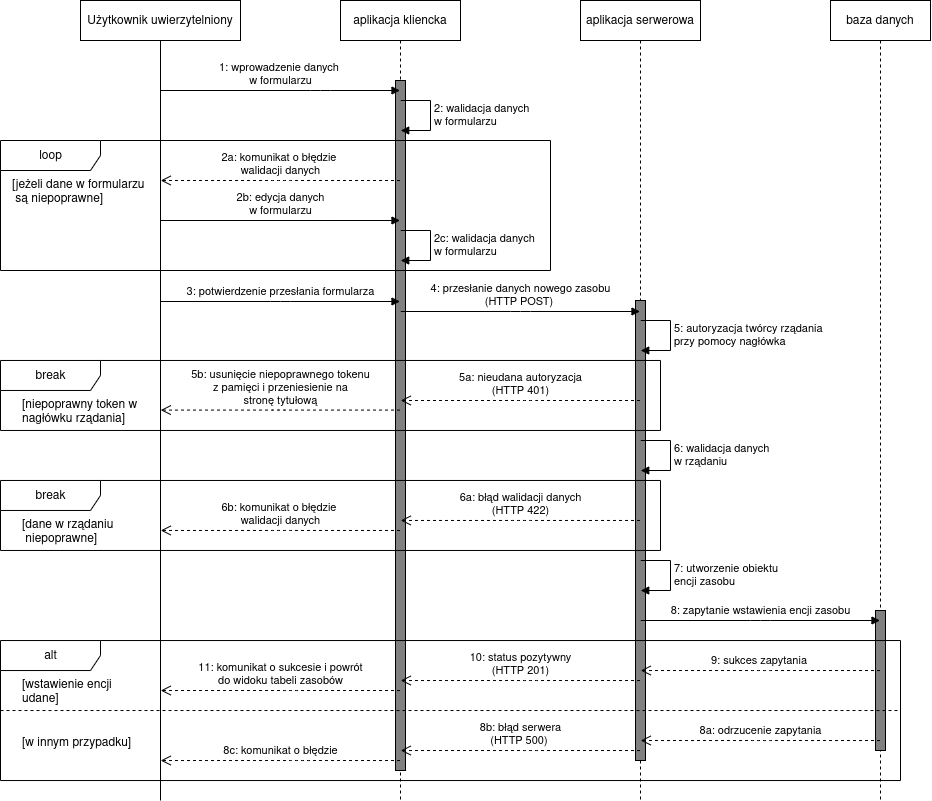
\includegraphics[width=\textwidth]{img/chapter4/open-osp.uml-diagrams-sequence.create-resource.png}
    \caption{Diagram sekwencji dodawania zasobu użytkownika}
    \label{fig:uml.sequence.create-resource}
\end{figure}

Jedynym aktorem, występującym w procesie, jest użytkownik uwierzytelniony, który dodaje przypisaną do niego encje zasobu w systemie. Warunkiem wstępnym jest, aby użytkownik korzystał od początku z widoku tworzenia nowego zasobu i posiadał token autoryzacyjny. Za warunek końcowy scenariusza, uznano sytuację, w której nowy zasób przypisany do użytkownika, został dodany do bazy danych systemu, a sam użytkownik został o tym fakcie poinformowany.

Główny przebieg zdarzeń opisany został w następującej kolejności:

\begin{enumerate}
    \item Użytkownik wprowadza w polach formularza tworzenia nowego zasobu, wartości jego atrybutów, wykorzystując aplikację kliencką.
    \item Aplikacja kliencka w sposób dynamiczny dokonuje walidacji danych w formularzu.
    \item Użytkownik potwierdza dodanie nowego zasobu przy pomocy przycisku przesłania formularza.
    \item Aplikacja kliencka wysyła żądanie HTTP metodą POST do interfejsu programistycznego aplikacji serwerowej. Żądanie zawiera dane nowego zasobu do utworzenia oraz token autoryzacyjny w nagłówku.
    \item Aplikacja serwerowa autoryzuje twórcę żądania przy pomocy przesłanego tokenu, sprawdzając między innymi jego ważność.
    \item Aplikacja serwerowa przeprowadza procedurę walidacji danych przesłanych w żądaniu.
    \item Aplikacja serwerowa tworzy obiekt encji zasobu, który zostanie zarejestrowany przez mechanizm mapowania obiektowo-relacyjnego.
    \item Aplikacja serwerowa przesyła do bazy danych zapytanie utworzenia nowej krotki w tabeli zasobów.
    \item W odpowiedzi baza danych przesyła komunikat o sukcesie zapytania.
    \item Aplikacja serwerowa wysyła do aplikacji klienckiej odpowiedź HTTP ze statusem 201, świadczącym o pomyślnym utworzeniu encji zasobu.
    \item Aplikacja kliencka informuje użytkownika o udanym utworzeniu przypisanego do niego zasobu.
\end{enumerate}

Wyróżniony został zakres zdarzeń opcjonalnych dla przypadku, w którym walidacja danych w kroku 2, wykryła niepoprawne dane wprowadzone w formularzu:

\begin{enumerate}
    \item [2a.] Aplikacja kliencka wyświetla komunikat o niepoprawnych danych wprowadzonych w formularzu.
    \item [2b.] Użytkownik edytuje dane w formularzu.
    \item [2c.] Aplikacja kliencka ponownie dokonuje walidacji danych. Jeżeli wprowadzone dane ponownie są niepoprawne, powtórzone zostaną zdarzenia 2a, 2b i 2c.
\end{enumerate}

W scenariuszu uwzględniono również niżej przedstawione zdarzenia alternatywne:

\begin{enumerate}
    \item [5a.] Ze względu na błąd autoryzacji, aplikacja serwerowa przesyła do aplikacji klienckiej odpowiedź HTTP ze statusem 401 (brak autoryzacji).
    \item [5b.] Aplikacja kliencka usuwa niepoprawny token z pamięci przeglądarki użytkownika i przenosi go do widoku strony tytułowej.
    \item [6a.] Aplikacja serwerowa wysyła do aplikacji klienckiej odpowiedź HTTP ze statusem 422 (niewykonalne żądanie).
    \item [6b.] Aplikacja kliencka informuje użytkownika o błędzie i prosi o ponowne uzupełnienie formularza.
    \item [8a.] Baza danych informuje o odrzuceniu zapytania utworzenia encji lub nie odpowiada aplikacji serwerowej. 
    \item [8b.] Aplikacja serwerowa przesyła aplikacji klienckiej informacje o błędzie wewnętrznym serwera przy pomocy odpowiedzi HTTP 500. 
    \item [8c.] Aplikacja kliencka informuje użytkownika o nieudanej obsłudze żądania.
\end{enumerate}

%%%%%%%%%%%%%%%%%%%%%%%%%%%%%%%%%%%%%%%%
\subsection{Edycja zasobu użytkownika}
%%%%%%%%%%%%%%%%%%%%%%%%%%%%%%%%%%%%%%%%

Proces edycji zasobu użytkownika zobrazowano diagramem na rys. \ref{fig:uml.sequence.update-resource}. Jedynym aktorem występującym w scenariuszu jest użytkownik uwierzytelniony. Zgodnie z warunkiem wstępnym, użytkownik na początku scenariusza korzysta z widoku edycji zasobu. Warunkiem końcowym jest, aby atrybuty edytowanego zasobu, zostały zaktualizowane w bazie danych systemu i użytkownik otrzymał komunikat o pomyślnie przeprowadzonej akcji.

\begin{figure}[!htbp] 
    \centering
    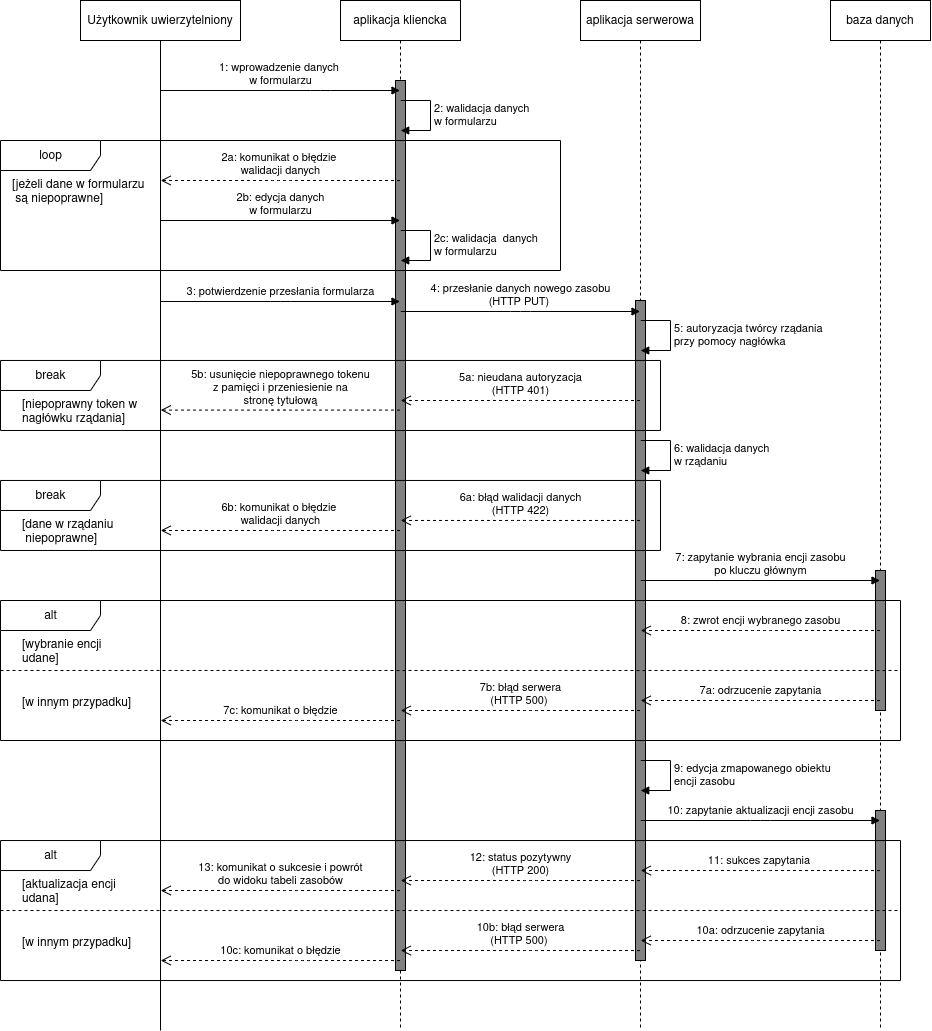
\includegraphics[width=\textwidth]{img/chapter4/open-osp.uml-diagrams-sequence.update-resource.png}
    \caption{Diagram sekwencji edycji zasobu}
    \label{fig:uml.sequence.update-resource}
\end{figure}

Poniżej wypunktowano główny przebieg zdarzeń scenariusza:

\begin{enumerate}
    \item Użytkownik wprowadza w polach formularza edycji zasobu, wartości jego atrybutów wykorzystując aplikację kliencką.
    \item Aplikacja kliencka w sposób dynamiczny dokonuje walidacji danych w formularzu.
    \item Użytkownik potwierdza edycje zasobu przy pomocy przycisku przesłania formularza.
    \item Aplikacja kliencka wysyła żądanie HTTP metodą PUT do interfejsu programistycznego aplikacji serwerowej. Żądanie zawiera nowe dane edytowanego zasobu oraz token autoryzujący w nagłówku.
    \item Aplikacja serwerowa autoryzuje twórcę żądania przy pomocy przesłanego tokenu.
    \item Aplikacja serwerowa przeprowadza procedurę walidacji danych przesłanych w żądaniu.
    \item Aplikacja serwerowa wysyła do bazy danych zapytanie wybrania istniejącej encji po kluczu głównym.
    \item Baza danych zwraca krotkę zasobu w odpowiedzi na zapytanie aplikacji serwerowej.
    \item Aplikacja serwerowa modyfikuje atrybuty encji poprzez edycje obiektu monitorowanego przez mechanizm obiektowo-relacyjny.
    \item Aplikacja serwerowa przesyła do bazy danych zapytanie aktualizacji krotki encji w tabeli zasobów.
    \item W odpowiedzi baza danych przesyła komunikat o sukcesie zapytania.
    \item Aplikacja serwerowa wysyła do aplikacji klienckiej odpowiedź HTTP z pozytywnym statusem 200. 
    \item Aplikacja kliencka informuje użytkownika o udanej modyfikacji zasobu.
\end{enumerate}

Jeżeli użytkownik wprowadził niepoprawne dane w formularzu, walidacja danych w kroku 2 nie powiedzie się, skutkując wystąpieniem opcjonalnych zdarzeń:

\begin{enumerate}
    \item [2a.] Aplikacja kliencka wyświetla komunikat o niepoprawnych danych wprowadzonych w formularzu.
    \item [2b.] Użytkownik edytuje dane w formularzu.
    \item [2c.] Aplikacja kliencka ponownie dokonuje walidacji danych. Jeżeli wprowadzone dane ponownie są niepoprawne, powtórzone zostaną zdarzenia 2a, 2b i 2c.
\end{enumerate}

Zdarzenia alternatywne, które mogą wystąpić w procesie edycji zasobu to:

\begin{enumerate}
    \item [5a.] Ze względu na błąd autoryzacji, aplikacja serwerowa przesyła do aplikacji klienckiej odpowiedź HTTP ze statusem 401 (brak autoryzacji).
    \item [5b.] Aplikacja kliencka usuwa niepoprawny token z pamięci przeglądarki użytkownika i przenosi go do widoku strony tytułowej.
    \item [6a.] Aplikacja serwerowa wysyła do aplikacji klienckiej odpowiedź HTTP ze statusem 422 (niewykonalne żądanie).
    \item [6b.] Aplikacja kliencka informuje użytkownika o błędzie i prosi o ponowne uzupełnienie formularza.
    \item [7a.] Baza danych informuje o odrzuceniu zapytania wybrania encji lub nie odpowiada aplikacji serwerowej. 
    \item [7b.] Aplikacja serwerowa przesyła aplikacji klienckiej informacje o błędzie wewnętrznym serwera przy pomocy odpowiedzi HTTP 500. 
    \item [7c.] Aplikacja kliencka informuje użytkownika o nieudanej obsłudze żądania.
    \item [10a.] Baza danych informuje o odrzuceniu zapytania aktualizacji encji lub nie odpowiada aplikacji serwerowej. 
    \item [10b.] Aplikacja serwerowa przesyła aplikacji klienckiej informacje o błędzie wewnętrznym serwera przy pomocy odpowiedzi HTTP 500. 
    \item [10c.] Aplikacja kliencka informuje użytkownika o nieudanej obsłudze żądania.
\end{enumerate}

%%%%%%%%%%%%%%%%%%%%%%%%%%%%%%%%%%%%%%%%
\subsection{Usuwanie zasobów użytkownika}
%%%%%%%%%%%%%%%%%%%%%%%%%%%%%%%%%%%%%%%%

Procedurę usuwania zasobów użytkownika zilustrowano przy pomocy diagramu sekwencji przedstawionego na rys. \ref{fig:uml.sequence.delete-resource}.

\begin{figure}[!htbp] 
    \centering
    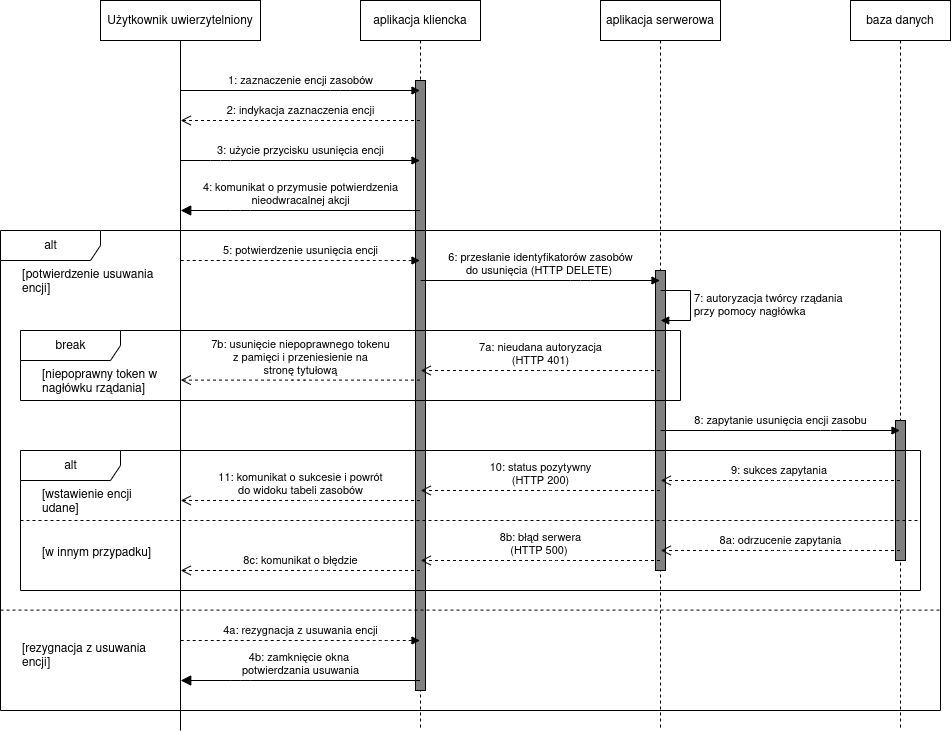
\includegraphics[width=\textwidth]{img/chapter4/open-osp.uml-diagrams-sequence.delete-resource.png}
    \caption{Diagram sekwencji usuwania zasobu}
    \label{fig:uml.sequence.delete-resource}
\end{figure}

Jedynym aktorem występującym w procesie jest użytkownik uwierzytelniony. Użytkownik wstępnie posiada token autoryzujący zapisany w pamięci przeglądarki i korzysta z widoku tabeli zasobów. Warunkiem końcowym jest natomiast trwałe usunięcie zasobu z bazy danych systemu.

Główny przebieg zdarzeń opisany został w następującej kolejności:

\begin{enumerate}
    \item Użytkownik zaznacza zasoby przy pomocy interfejsu aplikacji klienckiej.
    \item Aplikacja kliencka wyraźnie indykuje zaznaczenie zasobów.
    \item Użytkownik korzysta z przycisku usunięcia zaznaczonych zasobów.
    \item Aplikacja kliencka wyświetla widok potwierdzenia nieodwracalnego usunięcia zasobów.
    \item Użytkownik potwierdza zamiar usunięcia zaznaczonych zasobów.
    \item Aplikacja kliencka wysyła żądanie HTTP metodą DELETE do interfejsu programistycznego aplikacji serwerowej. Żądanie zawiera unikalne identyfikatory zasobów do usunięcia oraz token autoryzujący w nagłówku.
    \item Aplikacja serwerowa autoryzuje twórcę żądania przy pomocy przesłanego tokenu, sprawdzając między innymi jego ważność.
    \item Aplikacja serwerowa wysyła zapytanie usunięcia zasobów o przesłanych w żądaniu identyfikatorach.
    \item W odpowiedzi baza danych przesyła komunikat o sukcesie zapytania.
    \item Aplikacja serwerowa wysyła do aplikacji klienckiej odpowiedź HTTP ze statusem 200 świadczącym o pomyślnym skasowaniu zasobów z pamięci.
    \item Aplikacja kliencka informuje użytkownika o udanym usunięciu zasobów.
\end{enumerate}

Jako dopuszczalne zdarzenia alternatywne traktuje się:

\begin{enumerate}
    \item [7a.] Ze względu na błąd autoryzacji, aplikacja serwerowa przesyła do aplikacji klienckiej odpowiedź HTTP ze statusem 401 (brak autoryzacji).
    \item [7b.] Aplikacja kliencka usuwa niepoprawny token z pamięci przeglądarki użytkownika i przenosi go do widoku strony tytułowej.
    \item [8a.] Baza danych informuje o odrzuceniu zapytania usunięcia encji lub nie odpowiada aplikacji serwerowej. 
    \item [8b.] Aplikacja serwerowa przesyła aplikacji klienckiej informacje o błędzie wewnętrznym serwera, przy pomocy odpowiedzi HTTP 500. 
    \item [8c.] Aplikacja kliencka informuje użytkownika o nieudanej obsłudze żądania.
\end{enumerate}